%\documentclass[12pt,a4paper,twoside]{book} 
\usepackage[spanish]{babel} % de pedro
\usepackage{graphics,graphicx,epsfig,color,float,afterpage,fancyheadings,subfigure,moreverb,alltt} % de pedro
\usepackage[latin1]{inputenc} % tildes de pedro

\usepackage{algorithm}
\usepackage{algorithmic}

\usepackage{rotating}
\usepackage{url}

%% Esta letra se convierte mejor a pdf que la normal
\usepackage{ae}

%%% Para las fuentes matemticas
\usepackage{amsfonts}

\usepackage{subfigure}

\usepackage{pstricks} % para los dibujos del da
\usepackage{lscape} % para las pginas en horizontal
\usepackage{portland} % para las pginas en horizontal
\usepackage{supertabular} % para las tablas de ms de una pgina
\usepackage{tabularx} % para las tablas del tipo tabularx
%\usepackage{glossary}
%\documentclass[a4paper,spanish,12pt]{book} % esto es de gustavo
%\usepackage{amsmath,amsfonts}   % underset mathbb
%\usepackage{authordate1-4}      % bib style
%\usepackage{epsfig}     % eps
\usepackage{epic}           % graficos
%\usepackage{eepic}           % graficos
\usepackage{curvesls}           % curvas
\usepackage{amssymb}
%\usepackage{fancyheadings}  % encabezados
%\usepackage{hhline}             % hhline
%\usepackage[latin1]{inputenc}   % tildes
%\usepackage{makeidx}        % ndices
%\usepackage{setspace}           % interlinea
%\usepackage[spanish]{babel} % espaol

%%%%%%%%%%%%%%%%%%%%%%%%%%%%%%%%%%%%%%%%%%%%%%%%%%%%%%%%%%%%%%%%%%%%%%%%%%%%%%%

\author{juanlu}
\title{Tesis de Juan Lus Jimnez Laredo}




\newcommand{\fecha}{\footnotesize{[ Impreso: \the\day-\ifcase\month\or
    Ene\or Feb\or Mar\or Abr\or May\or Jun\or Jul\or Ago\or Sep\or
      Oct\or Nov\or Dic\fi-\the\year ]}}

\newcommand{\N}{\mathbb{N}}

%% Para corregir las cabeceras largas
\newcommand{\cabecera}[2]{
\markright{\ref{#1}. \hspace{0.1ex} \MakeUppercase{#2}}}


%\pagestyle{headings}
%\renewcommand{\chaptermark}[1]{\markboth{\fecha \\ \\ #1}{}}
%\renewcommand{\sectionmark}[1]{\markright{#1 \\ \\ \fecha}}
%\addtolength{\headheight}{2.5pt}



%\lhead[\it\thechapter]{\sl\rightmark}
%\rhead[\rm\leftmark]{\it\thesection}
%\rfoot[]{\thepage}
%\cfoot[]{}
%\lfoot[\thepage]{}

%\thispagestyle{plain}

\setcounter{secnumdepth}{3}
\setcounter{tocdepth}{3}

%\renewcommand{\baselinestretch}{1.2}
%\setlength{\parskip}{0.8ex}

\newtheorem{theorem}{\sf Teorema}
\newtheorem{lemma}{\sf Lema}

\newcommand{\rem}[1]{\S\iffalse #1 \fi}
\newcommand{\cur}[1]{ {\it #1\/} }
\newcommand{\crcl}[1]{#1\kern-9pt\raise1pt\hbox{$\bigcirc$}}
\newcommand{\evag}{{\sf EvAg}}
\newcommand{\evagp}{{\sf EvAg.}}
\newcommand{\evags}{{\sf EvAgs}}
\newcommand{\evagsp}{{\sf EvAgs.}}

\newcommand{\prog}[2] {
   \small
   \begin{minipage}[t]{75mm} {\tt #1}  \end{minipage}
   \begin{minipage}[t]{60mm} {#2}      \end{minipage}
   \\
}
\newcommand{\prg}[2] { {\tt #1} & {\sf #2} \\}

\newcommand{\wmfspecial}[4]{
   \begin{figure}[h]
   \centerline{\psfig{figure=#1,height=#2}}
   \caption{#3}   \label{#4}
   \end{figure}
}                   % USO: \wmfspecial{nombre.eps}{altura}{leyenda}{etiqueta}

\def\stackunder#1#2{\mathrel{\mathop{#2}\limits_{#1}}}

\def\marco #1#2#3#4{\centerline{       % USO: \marco{.1}{10}{124mm}
  \vbox{\hrule height #1pt%
  \hbox{\vrule width #1pt\kern #2pt%
  \vbox{\kern #2pt%
  \vbox{\hsize #3\noindent #4}%
  \kern #2pt}%
  \kern #2pt\vrule width #1pt}%
  \hrule height0pt depth #1pt}} }


\newcommand{\symnote}[2]{\symbolnote{#1}{#2}}

\newfont{\bi}{cmbxti10 scaled\magstep1}       % bf + it


%% Ruta de las figuras
\graphicspath{{../figuras/}}


\begin{document}
           % Eliminarlo al compilar el documento maestro, ponerlo para compilarlo separado

%%%%%%%%%%%%%%%%%%%%%%%%%%%%%%%%%%%%%%%%%%%%%%%%%%%%%%%%%%%%%%%%%%%%%%%%%%%%%%%
%%                                                                           %%
%%                             Tesis Doctoral:                               %%
%%                        Pablo García Sánchez                               %%
%%                                                                           %%
%%%%%%%%%%%%%%%%%%%%%%%%%%%%%%%%%%%%%%%%%%%%%%%%%%%%%%%%%%%%%%%%%%%%%%%%%%%%%%%

\cabecera{cap:p2pcompt}{Peer-to-Peer Computing} %Descomentarlo para compilar maestro
\chapter{\textit{Service Oriented Architecture}}
\label{cap:p2pcompt}
\cabecera{cap:p2pcompt}{Peer-to-Peer Computing} %Descomentarlo para compilar maestro

%%%%%%%%%%%%%%%%%%%%%%%%%%%%%%%%%%%%%%%%%%%%%%%%%%%%%%%%%%%%%%%%%%%%%%%%%%%%%%%

SOA es superguay porque...


\begin{figure}[htbp]
\centerline{\includegraphics[width=0.8\textwidth]{soahistory}}
\caption{La historia.}
\label{fig:spontaneous}
\end{figure}


\begin{figure}[htbp]
\centerline{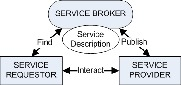
\includegraphics[width=0.8\textwidth]{soaDiagram}}
\caption{El dibujito basico.}
\label{fig:spontaneous}
\end{figure}

%%%%%%%%%%%%%% Bibliografia %%%%%%%%%%%%%%%

%\bibliographystyle{alpha}  % Eliminarlo al compilar el documento maestro, ponerlo para compilarlo separado
%\bibliography{p2pcomputing}%,gprop,mmitchell,zmich,hilera,fjmm,ripley,rbeale,jhertz,mag}       % Eliminarlo al compilar el documento maestro, ponerlo para compilarlo separado

%\end{document}             % Eliminarlo al compilar el documento maestro, ponerlo para compilarlo separado